\documentclass[a4paper,english]{article}

\usepackage[T1]{fontenc}
\usepackage[utf8]{inputenc}
\usepackage{graphicx}

\usepackage[a4paper, total={6in, 8in}]{geometry}
\usepackage{hyperref}
\usepackage{url}
\usepackage{breakurl}

\usepackage{caption}


% \title{Wanderer: integration and visualization of TCGA Data}
% \author{Anna D{\'i}ez-Villanueva, Izaskun Mallona and Miguel A. Peinado$^{**}$ \\
% \\
 % $^{**}$ Corresponding author
% }

% \date{\today}

\begin{document}

% \maketitle

% \begin{flushright}
% % \begin{figure}[]
%   \includegraphics[width=0.3\textwidth]{logo_imppc.png}
% % \end{figure}
% \begin{small}
% Ctra. de Can Ruti\\
% Camí de les Escoles s/n\\
% 08916 Badalona, Barcelona, España\\
% T 0034 93 554 3050\\
% www.imppc.org\\
% NIF G64351000\\
% \end{small}
% \end{flushright}

\hfill
\noindent
\parbox{4.5cm}{

\includegraphics[width=0.3\textwidth]{logo_imppc.png}
}
\begin{flushright}
\begin{small}
Ctra. de Can Ruti\\
Camí de les Escoles s/n\\
08916 Badalona, Barcelona, España\\
T 0034 93 554 3050\\
www.imppc.org\\
NIF G64351000\\
\end{small}
\end{flushright}
% }%


February 5th, 2015\\

Dear Editor,\\

We would like to inquire about the interest of Nature Methods  on a correspondence letter reporting a new web tool: Wanderer, an interactive viewer to explore DNA methylation and gene expression data in human cancer. The working version of Wanderer may be found at \burl{http://www.maplab.cat/betawanderer} (provisional address).\\

As you well know, The Cancer Genome Atlas (TCGA) initiative is an ambitious project aiming to accelerate our understanding of the molecular basis of cancer by providing large-scale genome information from thousands of clinically characterized cancer samples. The complex and comprehensive  nature of the generated data represents a privileged opportunity for researcher to get insights into the molecular landscapes of cancers. In fact, the landmark papers reporting the original data of each tumor type may just be considered a modest anticipation of the expected overall outcome. Nevertheless,  wet lab experimentalists have very limited access to these data because sophisticated bioinformatic skills are required to manage and analyze such large datasets. Hence, development of interfaces facilitating the visualization and analysis of the information to non-bioinformaticians is essential to get a broad exploitation of this gigantic effort.\\

As experimental researchers with a long track of investigations using both candidate oriented and exploratory type studies, we are fully aware of these shortcomings. Our response has been the development of Wanderer, a very simple and intuitive web tool allowing real time access and visualization of gene expression and DNA methylation profiles from TCGA data using gene targeted queries.\\

For any given gene selected by the investigator, the tool provides detailed individual profiles of gene expression, exon by exon, and DNA methylation of all the probes inside or in the vicinity of the gene (Figure \ref{fig:1}). Graphs for normal and tumor samples from any of the 19 available TCGA datasets are readily produced. Summarizing plots and tables are also generated, allowing further data analysis or representation using any software the investigator is used to (e.g.: Excel or any other spreadsheet or graphing tool). In addition, statistical analysis is applied to identify differential gene expression or DNA methylation between normal and tumor samples at either the single exon or the DNA methylation probe level, respectively. The tool allows local navigation and zoom in/out within the region of interest, as well as simple graph customization. Resulting graphs and tables may be downloaded and an application programming interface (API) allows data sharing, automatable query of multiple instances and direct linkage from external servers.\\
 
Some example of issues that can be resolved by querying Wanderer (and not easily reachable without this tool) include:
\begin{itemize}
\item Are different samples expressing the same gene isoforms? Which exon(s) should I analyze to find the largest difference between normal and tumor? See example in Figure \ref{fig:2}.
\item Which region of the CpG island should I analyze to find the largest abnormal DNA methylation in tumor samples? Is it the same for different tumor types? See example in Figure \ref{fig:3}.
\item Are methylation changes in the CpG island of my favorite gene specific? Or rather, are they consequence of a regional phenomenon? See example in Figure \ref{fig:4}.
\end{itemize}


While other web tools have been created to download, analyze and/or visualize TCGA data (e.g. cBioPortal, MethHC, UCSC Cancer Browser, Cancer Regulome, among others), no one of them offers similar features and with the simplicity of interface Wanderer has. We are convinced this tool will be very useful to wet lab researchers as they will easily improve the experimental design and select the target region with the highest interest for their specific objectives, with the concomitant savings in time and cost.\\

Looking forward for your reply.\\

Best regards.\\


Miguel A. Peinado\\
\noindent \href{mailto:map@imppc.org}{map@imppc.org}




\begin{figure}[center]
  \centering
  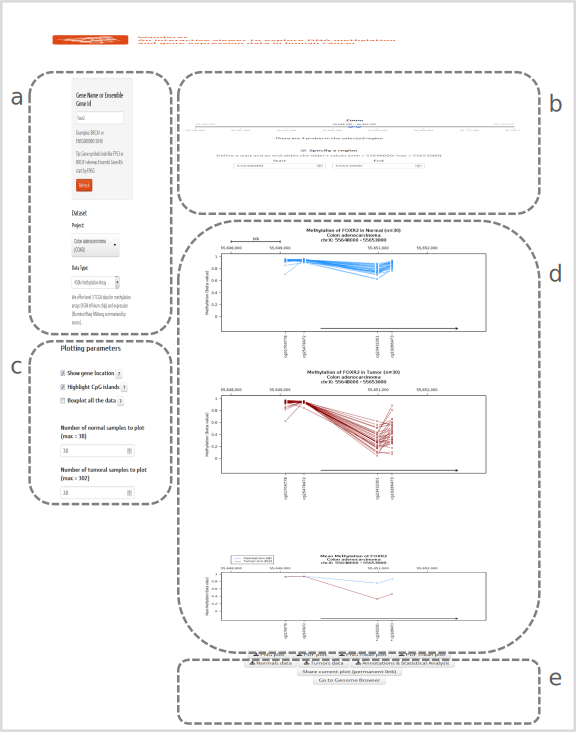
\includegraphics[width = \textwidth]{fig1.pdf}
  \caption{Snapshot of Wanderer webpage. Boxes indicate the different panels for gene name/ID and dataset selection (a), view customization (b and c), output (d) and data download and links (e). Web access to Wanderer: \href{http://www.maplab.cat/betawanderer}{http://www.maplab.cat/betawanderer}.}
  \label{fig:1}
\end{figure}




\begin{figure}[center]
  \centering
  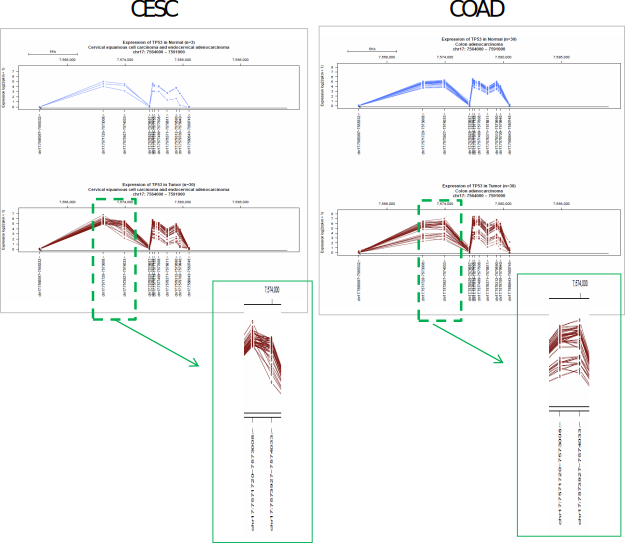
\includegraphics[width = \textwidth]{fig2.pdf}
  \captionsetup{singlelinecheck=off}
  \caption[Gene expression profile of TP53 in Cervical Squamous Cell carcinoma (CESC) and Colon adenocarcinoma (COAD).]{
    Gene expression profile of TP53 in Cervical Squamous Cell carcinoma (CESC) and Colon adenocarcinoma (COAD). TP53 expression levels are consistently reproduced among most exons in all COADs. In contrast, exon 11 reads counts do not reflect the variation observed in other exons in CESCs (see enlarged inset for comparison with exon 10).
    \begin{description}
    \item Gene: TP53
    \item Region displayed: chr17:7564000-7591000
    \item Datasets: Cervical Squamous Cell Carcinoma (CESC) and Colon carcinoma (COAD)
    \item Data Type: Illumina HiSeq RNA
    \item \textit{API access:}
    \item CESC: \burl{http://maplab.cat/betawanderer\_api?Gene=tp53&start=7564000&end=7591000&TissueType=cesc&DataType=expression&plotmean=FALSE&geneLine=TRUE&CpGi=TRUE&nN=3&nT=30}
    \item COAD: \burl{http://maplab.cat/betawanderer\_api?Gene=tp53&start=7564000&end=7591000&TissueType=coad&DataType=expression&plotmean=FALSE&geneLine=TRUE&CpGi=TRUE&nN=30&nT=30}
    \end{description}
}

  \label{fig:2}
\end{figure}





% \end{document}

% \begin{figure}[center]
%   \centering
%   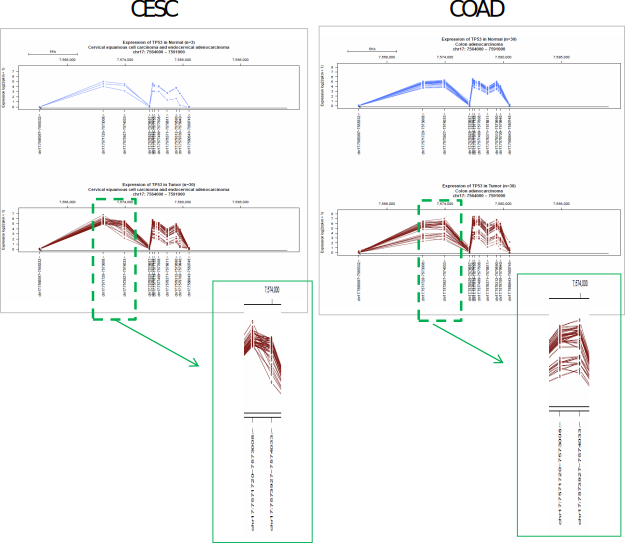
\includegraphics[width = 0.4\textwidth]{fig2.pdf}
%   \caption{

% Gene expression profile of TP53 in Cervical Squamous Cell carcinoma (CESC) and Colon adenocarcinoma (COAD). TP53 expression levels are consistently reproduced among most exons in all COADs. In contrast, exon 11 reads counts do not reflect the variation observed in other exons in CESCs (see enlarged inset for comparison with exon 10).\\

% \begin{itemize}
% \item Gene: TP53
% \item Region displayed: chr17:7564000-7591000
% \item Datasets: Cervical Squamous Cell Carcinoma (CESC) and Colon carcinoma (COAD)
% \item Data Type: Illumina HiSeq RNA
% \item API access:
% CESC: \href{http://maplab.cat/betawanderer_api?Gene=tp53&start=7564000&end=7591000&TissueType=cesc&DataType=expression&plotmean=FALSE&geneLine=TRUE&CpGi=TRUE&nN=3&nT=30}{http://maplab.cat/betawanderer\_api?Gene=tp53&start=7564000&end=7591000&TissueType=cesc&DataType=expression&plotmean=FALSE&geneLine=TRUE&CpGi=TRUE&nN=3&nT=30}

% COAD: \href{http://maplab.cat/betawanderer_api?Gene=tp53&start=7564000&end=7591000&TissueType=coad&DataType=expression&plotmean=FALSE&geneLine=TRUE&CpGi=TRUE&nN=30&nT=30}{http://maplab.cat/betawanderer\_api?Gene=tp53&start=7564000&end=7591000&TissueType=coad&DataType=expression&plotmean=FALSE&geneLine=TRUE&CpGi=TRUE&nN=30&nT=30}

% \end{itemize}
% }
%   \label{fig:2}
% \end{figure}


% \end{document}

\begin{figure}[center]
  \centering
  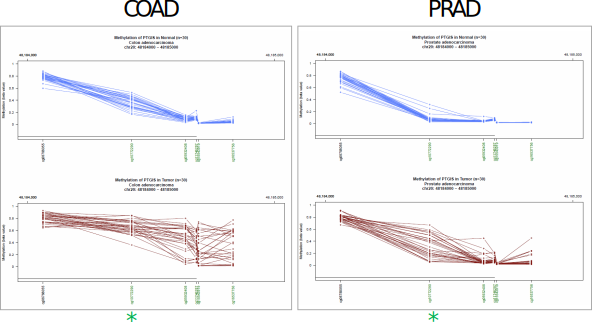
\includegraphics[width = \textwidth]{fig3.pdf}
  \captionsetup{singlelinecheck=off}
  \caption[DNA methylation profile of PTGIS CpG island in Colon adenocarcinomas (COAD) and Prostate adenocarcinomas (PRAD).]{
DNA methylation profile of PTGIS CpG island in Colon adenocarcinomas (COAD) and Prostate adenocarcinomas (PRAD). Note that cg1077290 probe (*) is already very methylated in colon normal tissue, offering poor discriminat resolution to detect tumor hypermethylation compared with the rest of CpG island probes (labeled in green). In contrast, this probe (cg1077290) shows the highest level of hypermethylation in Prostate cancers (PRAD) and remains unmethylated in normal, resulting as the most discriminant variable in tis type of cancer.\\
\begin{description}
\item Gene: PTGIS
\item Region displayed: chr20:48,184,000-48,185,000
\item Dataset: Colon Adenocarcinoma (COAD), prostate Adenocarcinoma (PRAD)
\item Data Type: 450K Methylation Array
\item \textit{API access:} 
\item COAD: \burl{http://maplab.cat/betawanderer\_api?Gene=ptgis&start=48184000&end=48185000&TissueType=coad&DataType=methylation&plotmean=FALSE&geneLine=TRUE&CpGi=TRUE&nN=30&nT=30} 
\item PRAD: \burl{http://maplab.cat/betawanderer\_api?Gene=ptgis&start=48184000&end=48185000&TissueType=prad&DataType=methylation&plotmean=FALSE&geneLine=TRUE&CpGi=TRUE&nN=30&nT=30}  
\end{description}

}
  \label{fig:3}
\end{figure}


% \end{document}

\begin{figure}[center]
  \centering
  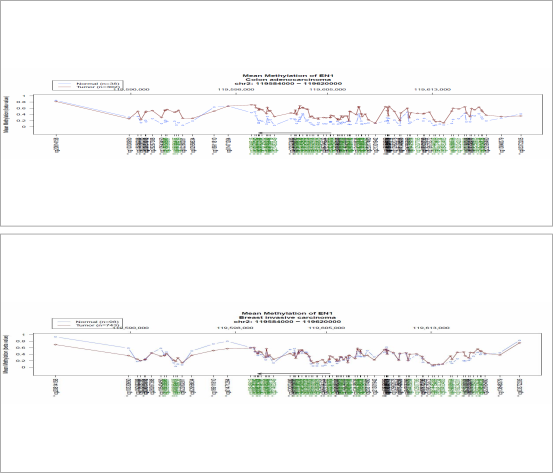
\includegraphics[width = \textwidth]{fig4.pdf}
  \captionsetup{singlelinecheck=off}
  \caption[DNA methylation profile of the genomic region flanking the EN1 gene.]{
DNA methylation profile of the genomic region flanking the EN1 gene. Note the large number of CpG islands (green probes) and that in Colon  adenocarcinomas (COAD),the whole region is hypermethylated, while in Breast cancer,  regions of hypomethylation and hypermethylation may be observed. The graphs display the average methylation values of each dataset. Probes marked with an asterisk denote statistically significant differences between normal and tumor samples.\\
\begin{description}
\item Gene: EN1
\item Region displayed: chr2:119,584,000-119,620,000
\item Dataset: Colon Adenocarcinoma (COAD), Breast Carcinoma (BRCA)
\item Data Type: 450K Methylation Array
\item \textit{API access}: 
\item COAD: \burl{http://maplab.cat/betawanderer\_api?Gene=en1&start=119507000&end=119657000&TissueType=coad&DataType=methylation&plotmean=FALSE&geneLine=TRUE&CpGi=TRUE&nN=30&nT=30}
\item BRCA: \burl{http://maplab.cat/betawanderer\_api?Gene=en1&start=119507000&end=119657000&TissueType=brca&DataType=methylation&plotmean=FALSE&geneLine=TRUE&CpGi=TRUE&nN=30&nT=30}
\end{description}


}
  \label{fig:4}
\end{figure}


\end{document}